\chapter{The ScienceIE Task: Design and Implementation}

To complete the ScienceIE task, a Java project was created containing three sub systems, each of which could be called independently. This section shall step through each subtask's design and implementation in order, beginning with a description of the preprocessing that was implemented, as it is generic to all subtasks. The following section shall describe the results associated with them.

\section{Data Preprocessing}
To support processing in later systems, all ScienceIE data had to be preprocessed. The idea of this piece of computation is to prepare the data for analysis, and to also reduce computation time as all systems can use this data (doing this process is done once rather than for each sub system). To further reduce experiment run time, Java serialisation was also used to save all the following preprocessing information for later retrieval.

In Java, for each paper file from ScienceIE, a \texttt{Paper} object was constructed. This held many important pieces of information about the paper in question, including location on disk, text extracted from its source file, and all preprocessing information. \texttt{Paper} itself is a \textit{plain old Java object}, only holding information and is an abstract class, with \texttt{TextPaper} and \texttt{PDFPaper} classes extending from it which could be instantiated. These extended classes inherited the data storage features and utilities from \texttt{Paper}, but their constructors are customised to extract information from their given type of file:

\begin{itemize}
	\item \texttt{TextPaper} is for \texttt{.txt} files and simply extracts the text from the document. It sees the title of the text document as the title of the paper.
	\item \texttt{PDFPaper} is for \texttt{.pdf} files. This uses Apache PDFBox\footnote{\href{https://pdfbox.apache.org/}{https://pdfbox.apache.org/} imported through Maven with \href{https://pdfbox.apache.org/2.0/dependencies.html}{https://pdfbox.apache.org/2.0/dependencies.html}} to extract the text from a PDF with the title being that of the document. As alluded to earlier, with the ScienceIE test set not only being just text files but also being short documents, longer PDF papers were not used, so little development to properly sanitise PDFs (removing titles, tables, etc...) happened, which would have been completed if this was the usual document format for this project.
	\item It was initially planned that there would be a \textit{HTML} and \textit{WebPDF} classes for online resources. For similar reasons to \texttt{PDFPaper} extraction development, these two classes were never implemented. 
\end{itemize}

The bulk of the preprocessing came in the form of using a parser to calculate the parse tree of a text, inspired by the projects at ScienceIE, to give later algorithms more information about the text to work with. As discussed, many teams at ScienceIE used spaCy. As the plan for this project was to complete it in a single, self contained Java project, the Stanford CoreNLP package was used \cite{Manning2014} (imported through Maven\footnote{\href{https://stanfordnlp.github.io/CoreNLP/download.html}{https://stanfordnlp.github.io/CoreNLP/download.html}}) which performs on similar analysis with similar quality to that of spaCy. While offering a range of useful NLP features, the main ones utilised by the project were tokenization and finding the parse tree of the text which included POS tagging. An \texttt{Annotator} class was constructed which accepts a \texttt{Paper} input and annotates the text using the CoreNLP library, with the result being stored in the \texttt{Paper}.

Further processing on this information was also completed: A token \textit{map} was created, with a key set being all tokens present in the document, and the value being the number of times the token was in the document. This was to help when calculating TF-IDF scores later in processing.

The final part of preprocessing was to load existing annotation information. Of course this was only possible for ScienceIE data, which were all supplied with the relevant \texttt{.ann} files in BRAT format. These records were loaded into a list of \texttt{Extraction} abstract entities, where each entry to the list could be either of a \textit{KeyPhrase} or \textit{Relationship} extending type, which each held all the information supplied in the annotation files.

\section{Subtask A - Key Phrase Extraction}
Subtask A at ScienceIE was considered the hardest, reinforced by both the maximum and average scores for each independent subtask. This paper dedicated most of its NLP effort to this task out of the three subtasks as this is currently the hardest part of information extraction (out of the given subtasks) given current research. 

Two attempts at this subtask were made. Initially, a \textit{safer} design involved a SVM which considers some of the key features about key phrases suggested in the literature around this topic. Then, a more experimental trail shall be described which involves clustering based around Word2Vec similarities between words in a document. 

\subsection{Method 1: Support Vector Machine}
Inspired by the highest success at ScienceIE, a SVM approach was adopted to attempt to provide a solution to subtask A. Initially, a small set of support vectors were selected and tested, with more being added as research continued.

\subsubsection*{Processing Data}
Two approaches were considered when designing the input and output data. One was based around passing each token in individually and in order, while the other was based around using the parse information obtained by using CoreNLP to pass sections of a sentence. 

Working with each individual token was selected for several reasons. Firstly, it was very easy to simply iterate through every token in a document in turn. Furthermore, the CoreNLP data can be used to describe individual tokens rather than truncated to summarize a sentence. While using sections of a sentence should help keep any key phrase extracted more semantically correct (i.e. it should avoid missing the end of a noun phrase), it poses a large issue: Any section selected as a key phrase would likely be \textit{locked down} as such to the specific tokens inside that section, meaning there may be no way to get rid of excess information or added extra if the gold standard key phrase requires something slightly different to the that chosen by the SVM. In terms of extra information needed, a system could be implemented to join adjacent key phrases but that would like see extra information over what is needed being included. If, to try and solve this issue, some system which could extend or shorten by token increments, the system would likely be very similar to processing individual tokens anyway. Therefore, a system based around processing each token individually was decided upon.

This resulted in a total of 65447 different training points (the number of individual tokens in the training data).

\subsubsection*{Defining Features}
It is clear that current trends view the position of key phrases are very important in the document and should definitely be considered when trying to learn how to predict them. A tokens proximity to other tokens semantically and as part of the document as whole seem to significantly help us identify where key phrases lie. Furthermore, some attributes about individual phrases also seem to play a large part. For example, the length of the word is a valid feature to evaluate, as the average length of a key phrase token (7 characters) is slightly different to the average of all key phrases (8 characters). 

\begin{table}
	\centering
	\caption[Initial Key Phrase SVM Features]{Initial key phrase support vector features used. A set of these features is generated for each token. When defining the value range, the variable is named as it is in the Java code.}
	\begin{tabular}{ C{7cm} | c }
		\textbf{Feature Description} & \textbf{Value Range} \\
		\hline
		The length of the token divided by the maximum token length in the training set. & \texttt{svLen} $\in$ $\mathbb{R}$,  0 $\leq$ \texttt{svLen} $\leq$ 1 \\
		\hline
     	Whether the token is a noun (using Part-Of-Speech tagging). & \texttt{svPos} $\in$ \{0, 1\} \\
     	\hline
     	The TF-IDF score of the token. & \texttt{svTfIdf} $\in$ $\mathbb{R}$,  0 $\leq$ \texttt{svTfIdf} $\leq$ 1 \\
     	\hline
     	The token index divided by the number of tokens. & \texttt{svDepth} $\in$ $\mathbb{R}$,  0 $\leq$ \texttt{svDepth} $\leq$ 1 \\
     	\hline
     	The token index in the current sentence divided by the number of tokens in the sentence. & \texttt{svDepthSentence} $\in$ $\mathbb{R}$,  0 $\leq$ \texttt{svDepthSentence} $\leq$ 1 \\
     	\hline
		Whether the token is in the first sentence of the paper. & \texttt{svFS} $\in$ \{0, 1\} \\
		\hline
     	Whether the token is in the last sentence of the paper. & \texttt{svLS} $\in$ \{0, 1\} \\
     	\hline
     	Whether the previous token was part of a key phrase. & \texttt{svLWKP} $\in$ \{0, 1\} \\
	\end{tabular}
	\label{table:kpinitsvs}
\end{table}

Thankfully, the idea behind using an SVM is to find what separates key phrases from just normal phrases. Therefore, an initial range of features was created, as defined in table \ref{table:kpinitsvs}. Here it is evident most of the features are based around trying to gather information as to the whereabouts of the token. It also considers the sequence of key tokens.

\subsubsection*{Training}
To train the SVM, a \textit{problem} must be created. The \textit{problem} contains an array of vectors, where the vector is the set of features described above. Each of these data points must be labelled. The label is what we are trying to predict on the test data, so here the label is where or not the token is a key phrase (\texttt{0} for \textit{normal}, or \texttt{1} for key phrase). 

\subsubsection*{Model Selection}
As the nature of the data is unknown, an educated guess can be made as to which kernel to use. A common kernel to begin working with is the \textit{Radial Basis Function} (RBF) kernel \cite{Chih-WeiHsuChih-ChungChang2008}. This is because it can handle non-linear data, which the training data here may be. The RBF kernel function to find the similarity between two data points is listed below:

\begin{equation*}
K\textsubscript{RBF}(x_i, x_j) = exp(-\gamma||x_i - x_j||^2)
\end{equation*}

\noindent There are two parameters which can be configured and tuned to optimise performance of the SVM:
\begin{itemize}
	\item $\gamma$, used in the RBF kernel. Values of the set \{0.25, 0.5 and 1\} shall be tested to investigate what works better, and to estimate whether decreasing or increasing this further may improve performance.
	\item The cost \textit{C} parameter. This influences the misclassification allowance, where a small value lets the SVM select a large hyper-plane for separating data but allows for more misclassification, and a large value should result in a small hyper-plane with little misclassification. Several values will be explored, of the set \{5, 50, 100, 200\}.
\end{itemize}

\subsubsection*{Development}
Having decided on how to use the concept of an SVM, there was a need for a concrete implementation. The idea of implementing an SVM was considered, however, with a responsibly high implementation complexity and a high risk of getting something subtly wrong (therefore being hard to detect and fix) a pre-existing solution was searched for. Furthermore, with the author having never handled an SVM before, a pre-existing solution with additional usage information was desired. This is why libsvm was chosen to be used in this project.

To allow for further SVM usage, an abstract \texttt{BaseSvm} was implemented so that any SVM created as part of this project could extend from this. This has a default configuration, a generic training method (calling \texttt{.svm\_train}), a generic predict method and a \texttt{.makeNewNode} method. This \texttt{.makeNewNode} method creates a feature for a data point in the format the SVM library can understand (a \textit{vector} is an array of \texttt{svm\_node}). It also validates the value of the feature, setting it to 0 is somehow an infinite or \textit{NaN} has been passed in. 

This \texttt{BaseSvm} class also holds a cross validation function (\texttt{.doCrossValidation(\textit{C}, $\gamma$)}), which runs the cross validation procedure and returns the accuracy as a percentage.

From the above, the \texttt{KeyPhraseSVM} class was created which contained the functionality to build the required feature vectors of input data and add labels to the training data, which completed the requirements of the SVM.

To actually produce \texttt{KeyPhrase} objects for a \texttt{Paper} object, once a token was \textit{predicted} to be part of a key phrase, its start and end position was noted. The following sequence of tokens would all have their predictions made, and while there is a string of tokens predicted to be key phrases, the end position is updated to cover this range of tokens in the original document. Once a token is predicted to not be a key phrase, the \texttt{.makeKeyPhrase} method of \texttt{Paper} is called with the start and end positions of the key phrase which returns the \texttt{KeyPhrase} object.

\subsubsection*{Additional Features and Post Processing}
While working on development of the key phrase SVM, further features were considered and implemented. To evaluate how effective they were, a baseline score was achieved and then each of these were added idea by idea to test if they increased the system performance or not. The additional items, in order, are listed in table \ref{table:kpextsvs}. 

\begin{table}
	\centering
	\caption[Additional Key Phrase SVM Features]{Additional features to be calculated for each token added to the SVM. These were implemented in order and their benefit or reduction in performance is measured.}
	\begin{tabular}{ C{7cm} | c }
		\textbf{Feature Description} & \textbf{Value Range} \\
		\hline
		The Word2Vec distance from the given token to ``task''. & \texttt{svTask} $\in$ $\mathbb{R}$,  0 $\leq$ \texttt{svTask} $\leq$ 1 \\
		\hline
		The Word2Vec distance from the given token to ``process''. & \texttt{svProcess} $\in$ $\mathbb{R}$,  0 $\leq$ \texttt{svProcess} $\leq$ 1 \\
		\hline
		The Word2Vec distance from the given token to ``material''. & \texttt{svMaterial} $\in$ $\mathbb{R}$,  0 $\leq$ \texttt{svMaterial} $\leq$ 1 \\
		\hline
		The depth of the token in the parse tree for its parent sentence, divided by the maximum depth of any token in that sentence. & \texttt{svParseTreeDepth} $\in$ $\mathbb{R}$,  0 $\leq$ \texttt{svParseTreeDepth} $\leq$ 1 \\
		\hline
		Whether or not the token is a stop word. & \texttt{svIgnoreWord} $\in$ \{0, 1\} \\
	\end{tabular}
	\label{table:kpextsvs}
\end{table}

The initial three focus on Word2Vec's \texttt{.similarity(word1, word2)} method, which finds the distance between two words in the Word2Vec space. The distances chosen were to the three types of classification laid out in the task description. The theory behind this is: as we are looking for tasks, processes and materials, words which are closely related to these concepts may be likely to have a higher similarity to those words in Word2Vec's vector space. Including this information as a feature in the SVM may help distinguish those data points which should be selected as key phrases (as they may be particularly close to one of the three target concepts).

Next, the parse depth of the token is considered. The idea of this is that if you imagine a parse tree, the leaves that are further away from the original sentence may generally be the more important parts of the sentence, as the other parts of the sentence (leaves less far down the tree structure) simply lead up to the key phrase and add extra information. Therefore, this should test to see if how \textit{central} a token is contributes to whether it should be seen as a key phrase.

Finally, there is a flag to described whether the token is a stop word. This should work with the TF-IDF feature described earlier to help identify words that are unimportant and should not be included in key phrases.

Along side these features, the results produced as part of development and manual analysis of the key phrases created gave incentive to apply some \textit{tidy up} through post processing. This was to remove unwanted parts of phrases or bad phrases entirely, and in conjunction with the above features the following post processes were applied:

\begin{itemize}
	\item \textit{TF-IDF filter} - In an attempt to remove key phrases which were effectively just \textit{noise}, each key phrase was treated as a candidate key phrase and would only become a true key phrase if the total TF-IDF of the tokens inside of it was above 0.02. This value was set by reviewing the key phrases produced in earlier runs, calculating their TF-IDF values, ordering them and finding the first key phrase contained non-stop words. The result was rounded down to the nearest hundredth and used as the filter.
	\item \textit{Sanitisation on creation} - The \texttt{.makeKeyPhrase} method was amended to only produce well formed key phrases. This includes attempting to remove redundant symbols, blank space and stop words at the start and end of the phrase. The goal was to try to reduce the gap between strict and inclusive evaluation by removing some of the redundant information. Consequently empty key phrases were also discarded.
	\item \textit{Final sanitisation changes} - The sanitisation added to the \texttt{.makeKeyPhrase} was revisited. The previous changes were refined and improved, and a new process added here was the splitting of key phrases if there is a bracket half way through the phrase. This creates two, more semantically correct key phrases (as originally, either side of the bracket would have been from different parts of the sentence), where at least one is more likely to be correct as no gold standard key phrase go across a bracket boundary. 
\end{itemize}

Through some analysis of the output, the final changes to sanitisation also gave this system the opportunity to match obvious synonyms: If the original key phrase was ``Support Vector Machine (SVM'', the two split phrases would be ``Support Vector Machine'' and ``SVM''. A simple check was implemented to see if the capitalised characters of the first phrase (``Support Vector Machine'' would be filtered to ``SVM'') were part of the second and vice versa, and if so a synonym relation was drawn between the pair of key phrases. 

\subsubsection*{Cross Validation}

\begin{figure}
	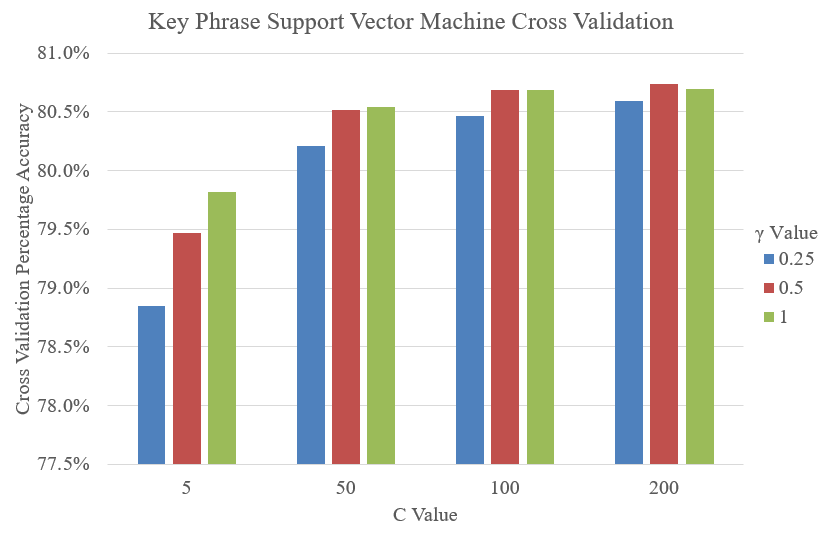
\includegraphics[width=\textwidth]{img/kpsvmcrossvalidation.png}
	\caption[Key Phrase SVM Cross Validation]{The cross validation results on the key phrase SVM. These were completed with all initial features and all extension features in place.}
	\label{figure:kpsvmcv}
\end{figure}

Cross validation is important when trying to optimise performance of an SVM. It allows for tuning key parameters by running repeated tests. Rather than tuning to optimise performance on the test data, which would introduce bias, the training data is split up into \textit{n} folds (or groups of data from within the training set). \textit{n = 5} folds were used in this instance. In turn, the SVM is trained with 4 of the 5 folds and then evaluated against the remaining fold. This is repeated for all combinations of folds and the average accuracy of the SVM can be calculated. A higher accuracy should mean better performance, although there is the problem of over fitting to consider. If the model is built to run perfectly on the training data, real world performance may actually suffer. This is why we cannot stop testing the SVM after just cross validation, as evaluating against the unseen test set will tell us how well it really performs. 

The values discussed for \textit{C} and $\gamma$ were used in cross validation and their outputs compared. The cross validation results can be seen in figure \ref{figure:kpsvmcv}. As show by this chart, very little change is accuracy is observed. There is a upward trend as \textit{C} and $\gamma$ increase, but this appears to plateau as higher values are evaluated. No smaller values need testing as (given the trend continues) the accuracy will significantly diminish. In terms of increasing the values, there is potential for extremely small gains; however, the return from this will be almost worthless and the training time required as the \textit{C} value increase significantly rises, as the SVM is working harder to find a better fitting hyperplane. Therefore, \text{C = 100} and \textit{$\gamma$ = 0.5} shall be used when completing full experiments. While, a \textit{C} value of 200 is 0.05\% more accurate with the same $\gamma$ value, the training time is roughly doubled (from some hours to many hours) and the reward is not deemed worth it.

\subsubsection*{Self Evaluation}
A problem referenced in the literature review was evaluation of key phrase extraction. What was discussed is how to classify good and bad systems. It is easy to accurately say how well a system performed compared to a set of gold standard data, but this paper considers whether that is enough to say whether a given extraction system is a success or not.

\begin{table}
	\centering
	\caption[Strictness Descriptions for Self Evaluation of Key Phrases]{The strictness levels used in self evaluation of key phrase extraction. The \textit{strictness} title also includes the \texttt{Strictness} enumeration value as in the Java code for reference.}
	\begin{tabular}{ C{3cm} | C{10cm} }
		\textbf{Strictness} & \textbf{Description} \\
		\hline
		Very strict (\texttt{REALLY\_STRICT}) & Both the predicted key phrase string and its boundaries need to match the gold standard string and boundaries. This is of equivalent strictness to the ScienceIE evaluation. \\
		\hline
		Matching (\texttt{STRICT}) & Just the predicted key phrase string needs to match the gold standard string. \\
		\hline
		Inclusive matching (\texttt{INCLUSIVE}) & The predicted key phrase string must be equal too or include the gold standard string. \\
		\hline
		Generous matching (\texttt{GENEROUS}) & The predicted key phrase string can include the gold standard string, or the gold stand string can include the predicted. \\
	\end{tabular}
	\label{table:strictness}
\end{table}

Therefore, in preparation for evaluation, several metrics will be used. The metric titles and descriptions can be seen in table \ref{table:strictness}. The point of these different metrics for deciding whether a prediction is good or not, is to capture a sense of how much of the gold standard information is being extracted, potentially allowing for some extra information. Of course, a metric equal to that of the ScienceIE test scripts is included so an expected value for when running with those scripts can be found, which also gives a good comparison value for the other metrics used in this paper.

Firstly, the \textit{matching} variant is believed to be perfectly reasonable: it results in exactly the same textual information output, it is merely less concerned with the informations original location. A higher score in this should be considered very positive, as when a reader is looking through key phrases extracted from various papers (for example when trying to pick one out that is useful to them), they likely don't care exactly which sentence the text came from. Even when looking at an individual paper as part of the ScienceIE data set, origin sentence likely doesn't matter as the documents are short and it should be easy to see where the phrase could have come from. This relaxed metric compared to the ScienceIE evaluation may be less favourable if the data set was made up of larger documents, as position in a large document makes more of a difference if trying to find information surrounding a key phrase; however, here it should be reasonable to just check successful key phrase extraction in this way.

There are also two much more lenient metrics. While it is not thought these should be official ways to evaluate an extraction technique, it is worth considering what these metrics are telling us about what information has been extracted. Evaluating with the \textit{inclusive} metric will inform the reader about how many of the key pieces of information have been found, but potentially with some extra information included. This extra information lowers the quality of the key phrases, but does not stop the key pieces of information from being extracted. Therefore, if using this metric scores a high result, the extracted pieces of information is likely still very useful, even if stricter metrics return significantly lower results. The \textit{generous} metric is less useful, as it will likely allow many false positive \textit{true positives} through an evaluation system - given a \textit{true positive} can be awarded when just part of a key phrase is extracted - which does not guarantee key words within the key phrase are captured. However, similar \textit{inclusive} and \textit{exclusive} scores that are both high should mean there are very few instances where only part of a key phrase has been captured, while most key phrases predicted are correct, or have some extra information attached.

The evaluation described above shall be used to evaluate SVM progression as each extension is added, with the \textit{best} SVM version found there used when testing on the ScienceIE scripts.

\subsection{Method 2: Clustering}
\subsubsection*{Concept}
Clustering has been shown to be effective in key phrase and other information extraction. A seemingly effective method was using \textit{term relatedness} to group terms, and then find an exemplar term at the centre of the clusters which can be used as a key phrase \cite{Liu2009}. 

Inspired by this, this paper proposes a similar process, where the similarity of terms is based around their Word2Vec similarities. Conceptually, it is possible that gathering similar terms will have the effect of creating clusters of important concepts, from which key phrases can be extracted. With the most similar words at the centre of clusters, these could be considered key words which are used to take a key phrase from the document. This should also exclude unimportant or stop words, as these shouldn't be close to significant concepts. In the study references, a filter was used to also remove some of these \textit{noisy} words, which shall also be used here.

An important note here is that the document is treated as a \textit{bag-of-words}, where we ignore the semantic meaning of the words. Word2Vec does this anyway, as when using the library the word is simply passed as plain text with no extra information, and Word2Vec uses its own ideas about the words semantic meanings to evaluate it. Using a bag-of-words approach means words from any part of the document could be clustered together, which is ok as if both are close to the centre of a cluster, it may mean both of them are key phrase worthy and should be selected.

The clustering algorithm selected was hierarchical clustering \cite{Rai2010}. Bottom up (agglomerative) hierarchical clustering works as follows:
\begin{enumerate}
	\item Each element begins in their own cluster (so \textit{n} elements means initially there are \textit{n} clusters).
	\item Given some distance metric, the distances between all clusters are calculated.
	\item The closest two clusters are combined.
	\item This process is repeated until a single cluster is left.
\end{enumerate}
\noindent This algorithm was chosen for several reasons:
\begin{itemize}
	\item It has a relatively low implementation difficulty.
	\item While the term similarities are based off of Word2Vec similarities, the distances between clusters could be evaluated in a number of ways. These include \textit{single} (the shortest distance between terms in two clusters), \textit{average} (the average distance between clusters) and \textit{complete} (the largest distance between terms in two clusters). These are called the \textit{linkage criteria}.
	\item If successful, this may aid in classification, as well as key phrases. After extracting key phrases, clustering could continue to form three clusters, each one potentially being a different classification (but will only work if initial extraction is successful). If doing this clustering was purely for classification, k-means clustering may be more appropriate with \textit{k = 3} to target the number of classifications.
\end{itemize}

When working with hierarchical clustering, an important aspect to consider is how far to iterate through the algorithm. In theory, the algorithm should run until there is just one cluster left with every element in it - but this is not useful. The more useful cluster states will be part of the way along the iterative cycle. To find this \textit{sweet spot} will require manual tuning, via inspecting the progression of the clusters to try to identify a good range where key phrase information can be extracted. In theory finding the sweet spot could be automated and learnt but to fully develop this kind of system would require a lot of time, which is very expensive.

A large difference between this and SVM usage is that this method is unsupervised learning and does not require training data, while using an SVM is supervised learning. This means that, given this method works for this testing scenario, its application may scale better in the \textit{real world} as is it not tied to the quality of the training data. Furthermore, given a suitable Word2Vec model, differences in key phrase output may be seen. This means that this algorithm may suffer here given the Word2Vec models currently available are not based on scientific publications, but running this algorithm on test data with similar context to the Word2Vec model may improve things, which means it may even cope with different languages.

\subsubsection*{Development}
The process of turning this theory into a practical implementation is straight forward. To allow for future expansion if clustering was to be used again for anything, a generic abstract \texttt{Cluster} class was created, which was formed of a list of items and declaration of functions to find the distance between a given cluster object and another cluster, and to create a new cluster by combining a given cluster object with another. A \texttt{Linkage} enumeration was created which could be used when testing to specify the method for finding the distance between two clusters.

The actual clustering begins by splitting the document into all of its tokens, removing duplicates. Then, stop words and unimportant words are removed. Unimportant words are classified based on their TF-IDF scores. All words were sorted according to their TF-IDF score, and the bottom 15\% were seem as noise and removed. This percentage was manually set, after generating this data and evaluating where the cut off should be to remove all words that are not in any key phrase and that are all stop words. Care was needed when setting this threshold, as for example ``results'' has a low TF-IDF score of 0.006 but is in the key phrase ``generalization of these results to the NSI case''. Of course, that phrase also includes other words like ``of'' and ``the'' which would be removed, but when we have some key words we could then reintroduce the semantic information and try to form well formed snippets, meaning stop words could be included in key phrases despite not being clustered. Therefore, 15\% was found to be a reasonable compromise to remove the particularly low TF-IDF valued tokens and to leave the more interesting tokens in the bag-of-words.

Then, the process of hierarchical clustering happens as described above. This happens for all test data, with all three linkage methods, with results being saved to disk. The output is then evaluated on a sample of the processed documents (as manually reviewing all 100 documents cluster patterns across 3 different linkage criteria is too much for a single reviewer to achieve) to evaluate if and where key phrases can be extracted.

\section{Subtask B - Key Phrase Classification}
\subsection{Word2Vec Usage}
With a large amount of influence coming from Word2Vec, the decision was made to focus on exploiting this technology to try to classify key phrases.

As the whole concept of Word2Vec is word similarities based on their semantic meaning, the idea is proposed that simply examining the distance from a key phrase to the relevant classification term or similar may result in a reasonably accurate classification. 

An important thing to consider is that Word2Vec generally accepts individual tokens. This contrasts to what we are trying to classify which is a string of tokens. Therefore, a way to find the similarity between a string of tokens and a singular token must be devised.

Two methods for achieving a distance metric are proposed and shall be tested:
\begin{itemize}
	\item Average distance, based on each token in the phrase and the target token,
	\item Shortest distance, being the closest token in the phrase to the target token (highest value in terms of \textit{similarity}).
\end{itemize}

There is also the problem of token importance as not all tokens will aid in classifying a key phrase. For example, ``determine the lowest energy configuration'' has the word ``the'' as a token. This token is bad as it is a likely word for any classification. Therefore, it is theorised that stop words being removed could help improve classification results.

There is a potential downside to this, as some key phrases may appear as only containing stop words. ``He'' for example is a key phrase (a synonym of ``helium''), but it would be seen as a stop word and remove. In this case it would actually nullify the key phrase, meaning no classification can be generated. Hence this algorithm should be tested with and without unimportant words being removed, as not all of them may actually be unimportant.

\begin{table}
	\centering
	\caption[Word2Vec Classification Target Words]{The target classes and the set of words that are of a similar domain to be used in testing of the Word2Vec classifier.}
	\begin{tabular}{ c | c }
		\textbf{Target Class} & \textbf{Similar Word Set to use when Testing} \\
		\hline
		Task & Task, Application, Goal, Problem \\
		 \hline
		Process & Process, Model, Algorithm\\
		 \hline
		Material & Material, resource \\
	\end{tabular}
	\label{table:w2vclasswords}
\end{table}

Finally, there is the question of what token to find similarity too. A simple way forward is comparing the tokens to the word identifying the class (``test'', ``process'' and ``material''). However, if the quality of the Word2Vec model isn't very good (it could have an incorrect idea about what a \textit{task} is for instance) the classification may be of poor quality as well. To attempt to solve this problem, more words based around the same concept should be tested against. Therefore, when testing this algorithm the similarities used will be the similarity of the word defining a class, or the maximum similarity to a word from a selection of words related to a class. The words sets that shall be used are defined in table \ref{table:w2vclasswords}.

\subsubsection*{The Word2Vec Vocabulary Problem}

\begin{figure}
	\centering
	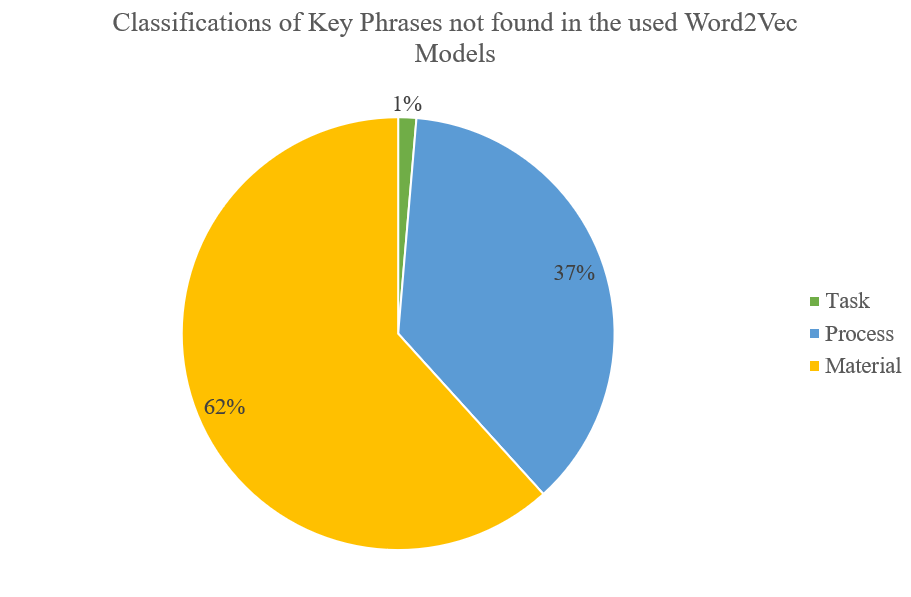
\includegraphics[width=12cm]{img/w2vbadtokensclasses.png}
	\caption[Key Phrase Classifications not in Word2Vec Model]{Gold standard key phrase classifications for key phrases that are not in the Word2Vec models used. 222 key phrases are included in this set.}
	\label{figure:w2vbadtokensclasses}
\end{figure}

An anticipated problem, proven through early testing, was that not every token in the scientific papers supplied by ScienceIE appeared in the Word2Vec models, and are therefore unclassifiable. Applicable tokens in the ScienceIE test set were checked to see their original classification, the result of which can be seen in figure \ref{figure:w2vbadtokensclasses}. Almost two thirds of these phrases are \textit{materials}. Therefore, a default class of \textit{material} will be assigned.

A model using the ScienceIE training data was created and tested (to create a more context appropriate model), however the low quantity of data saw extremely inaccurate results.

\subsection{Development}
As the design of this classifier is only concerned about classifying one key phrase at a time, and Word2Vec only accepts strings, the only piece of information needed to run the classifier is the key phrase string. Therefore, only one public method needs to be exposed as part of the library to do this classification, requiring the key phrase string and the Word2Vec model. The class implemented has no need to be stateful (as the method simply takes all it needs as parameters) so the implemented \texttt{W2VClassifier} cannot be instantiated and contains only \texttt{static} methods. For testing purposes, extra parameters are able to be passed to configure how is it run (many words, remove stop words, etc.).

Upon calling the method, the key phrase string is split into its individual tokens. These tokens are then individually checked, firstly to see if they are a stop word, and then to ensure they are actually in the Word2Vec model (with the convenient \texttt{.hasWord(word)} method). Given a token passes both of these checks, its similarity to the target word (or words) for each classification is found and either averaged with the other token similarities in that key phrase, or compared to the current maximum similarity found for that phrase and selected if larger. To find this similarity, Word2Vec has a \texttt{.similarity(word1, word2)} method, which returns the cosine similarity of the two words in vector space. 

This similarity metric is calculated for each type of classification. Upon finishing checking each phrase, these values are compared and the largest one selected, and the classification it represented returned (a \texttt{Classification} enumeration is used). If all of the similarity values are 0, no token in the phrase passed the initial checks; meaning we cannot classify the key phrase and therefore must return a default value.

\section{Subtask C - Relation Extraction}
\subsection{Word2Vec Usage}
Having considered Word2Vec's similarity function in the previous subtask, it shall again be utilised for this subtask. The goal here is to find relationships between key phrases, that can be categorised as hyponym (\textit{is-a}) and synonym (\textit{same-as}) relationships. 

To achieve this, we consider the relative distances tokens in a Word2Vec vector space hold to each other. In theory, if words A and B, of the same type of nature (for example cities), are semantically connected in the same way to words C and D, of the same type of nature (for example countries), respectively, the relative distance between A and C should be very similar to that of B and D. It should also stand that the relative distance A to B is similar to C to D. 

Therefore, the experiment here is to test if pairs of items that are synonyms share approximately the same relative distances between each other, and the same for hyponyms. The hope is to find a way to match synonym distances and hyponym distances. 

To achieve this, as usage of support vector machine was leveraged in subtask A, it shall again be used here to construct a system that can interpret the relative distance information produced by Word2Vec for given pairs of key phrases. Two proposed ideas for feature sets based off of the Word2Vec vector information, and their development, are presented below.

\subsection{SVM - Many Features}
The first attempt at constructing a SVM to interpret the meaning of Word2Vec distances shall be based on the literal vector space difference. The vector spaces in the model have dimension sizes of 300 and 1000 for Google News and Freebase respectively. As 1000 is extremely large, and Google News has a larger vocabulary than the Freebase model, this experiment will only work with the Google News Word2Vec model. Therefore each item added to the support vector machine shall have 300 features. 

The features shall be the difference between two key phrases' vectors, taken from Word2Vec. Word2Vec has a method, \texttt{.getWordVector(word)}, which returns the vector of a given word in Word2Vec space. With two vectors representing two key phrases, one vector can be subtracted from the other, and this is a data point.

Of course, as described in subtask B, Word2Vec cannot take a string of words, so instead we process each token of a phrase individually, summing their vectors as each is processed. Furthermore, it is possible that some tokens in a key phrase are not significant to a phrase, so these can be removed. Three variants on calculating the final vector of a key phrase are proposed:
\begin{itemize}
	\item Summing the Word2Vec vector representation of all tokens in a key phrase,
	\item Removing stop words and summing the vectors of the remaining tokens (if this nullifies phrases as discussed in subtask B, the algorithm reverts the above calculation),
	\item Using the parse information about the phrase to attempt to extract the root noun from it. Not all key phrases have nouns, and when this happens all tokens are summed together, but as the overwhelming majority of them do have a noun, using just that token seems sensible as it is likely the key part of the phrase.
\end{itemize}

To generate the training data, all key phrases were paired with all other key phrases (within their papers). The vector differences were all calculated, and the key phrase pairs that were hyponym or synonym relations labelled. Rather than one SVM that handled multiple labels, two SVMs were trained, one with the hyponyms labelled and the other with synonyms labelled. The thought behind this was that it would be simpler to manage training and testing as hyponyms and synonyms could be dealt with separately. As with the key phrase SVM, the RBF kernel was once again used.

Cross validation was applied to both SVMs, however, the range of values tested did not seem much change. The top row of figure \ref{figure:relsvmcv} show the cross validation results for this set of SVMs, and do not really indicate any trend. For both hyponym and synonym of extraction, \textit{C = 5} and \textit{$\gamma$ = 1} appeared to have slightly higher accuracy, but overall very little difference can be seen. The reason the accuracy is extremely high (all results are less than 0.5\% from 100\%) is because of the low amount of \textit{true case} relationship training points compared to the whole data set: 674 total relations out of 144410 possible combinations. This may prove problematic when testing on real world data, as the SVM effectively has a lack of good training data to learn off of (so may struggle to fit a good separating hyperplane).

This \textit{many features} SVM was implemented in \texttt{RelationshipSVM} (which extends from the previously described \texttt{BaseSvm}).

\begin{figure}
	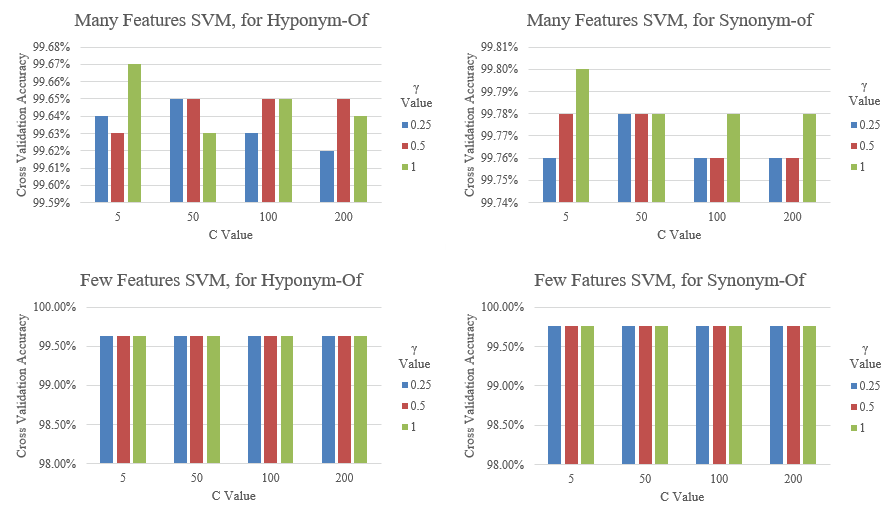
\includegraphics[width=\textwidth]{img/relsvmcrossvalidation.png}
	\caption[Relation SVM Cross Validation]{The cross validation results on both the hyponym and synonym variants of the \textit{many features} and \textit{few features} relationship SVMs.}
	\label{figure:relsvmcv}
\end{figure}

\subsection{SVM - Few Features}
Mentioned above, as the data was sparsely labelled and each point had a high feature count in the \textit{many features} SVM approach, this \textit{few features} approach aimed to reduce the complexity of the data presented in a hope it would allow for easier hyperplane fitting, meaning significantly reduced training times and hopefully a higher accuracy rate.

The idea was to reduce the vectors generated by Word2Vec to retain much of the same information in a simpler format. The result of this idea was to generate, given two key phrase vectors, the angle and the distance between the two vectors. The reason for these two metric is because these should preserve relative differences between vectors, as it is still based on the change in vector space between them.

To achieve this, the algorithm for generating a data point initially generates a vector sum of the tokens in each key phrase. With the two vectors prepared, the following was calculated:
\begin{itemize}
	\item Euclidean distance between the two vectors:
	\begin{equation*}
	d(\overrightarrow{u}, \overrightarrow{v}) = ||\overrightarrow{u} - \overrightarrow{v}|| = \sqrt{(u_1 - v_1)^2 + (u_2 - v_2)^2 ... + (u\textsubscript{300} - v\textsubscript{300})^2}
	\end{equation*}
	\item The angle between the two vectors based on the dot product:
	\begin{equation*}
	cos(\theta) = \dfrac{\overrightarrow{u} \cdot \overrightarrow{u}}{||\overrightarrow{v}|| \cdot ||\overrightarrow{v}||}
	\end{equation*}
\end{itemize}

These two values are then used as the features of each data point. A point is generated per pair of key phrases in a document, and labelled as to whether or not they are a relation. As with the \textit{many features} version, two SVMs were trained, one for hyponyms and one for synonyms, both using the RBF kernel.

Unfortunately, completing cross validation for this \textit{few features} SVM approach was not fruitful. The result can be seen in figure \ref{figure:relsvmcv}, with the relevant charts below that of the \textit{many features} cross validation results. Across the board for both SVMs, there is no change is accuracy with the different values tested. This likely means that no selection of relations is happening (the high accuracy is again because most of the data points should not be labelled as relationships), which does not bode well for real world tests. Given there is no visible trend, it is hard to evaluate how tune the SVM further to improve standings. Theoretically, increasing the \textit{C} value may allow for the SVM to find a better hyperplane which may help, but with when \textit{C = 200}, the training time is many hours and the development computer does not have enough memory to train further than that. 

This \textit{few features} SVM was implemented in \texttt{RelationshipSVM2} (which also extends from \texttt{BaseSvm}).
